\chapter{Einleitung}
\label{sec:einleitung}

Einleitender Text

\section{Motivation}

Beschreibung der Motivation, siehe Abbildung~\ref{fig:LampFlowchart}.

%Grafik aus PNG-File - bei dieser Variante darauf achten, dass die Grafik in ausreichender Auflösung vorliegt (so dass auch nach Skalierung >300dpi im Ausdruck erreicht werden)
\begin{figure}[htb]
  \centering
  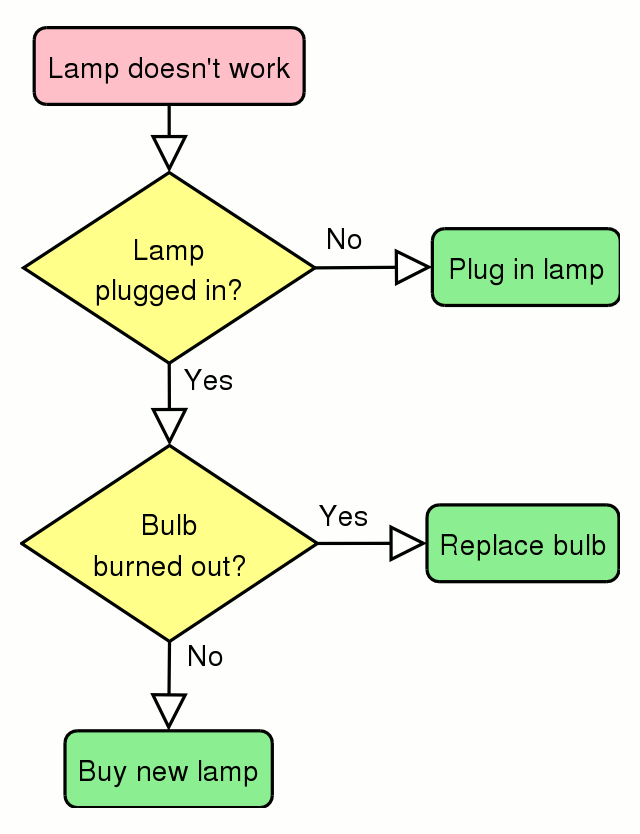
\includegraphics[width=.4\textwidth]{LampFlowchart}\\ % PNG-File
  \caption{Nulla interdum aliquam leo}\label{fig:LampFlowchart}
\end{figure}


\section{Ziele der Arbeit}

Ziele der Arbeit (vgl. Abbildung~\ref{fig:BurgerFlowchart}). Als Bonus können auch Forschungsfragen formuliert werden.

%Grafik aus PDF-File - diese Variante ist vorzuziehen, da sie die Einbundung echter Vektorgrafiken ermöglicht
\begin{figure}[htb]
  \centering
  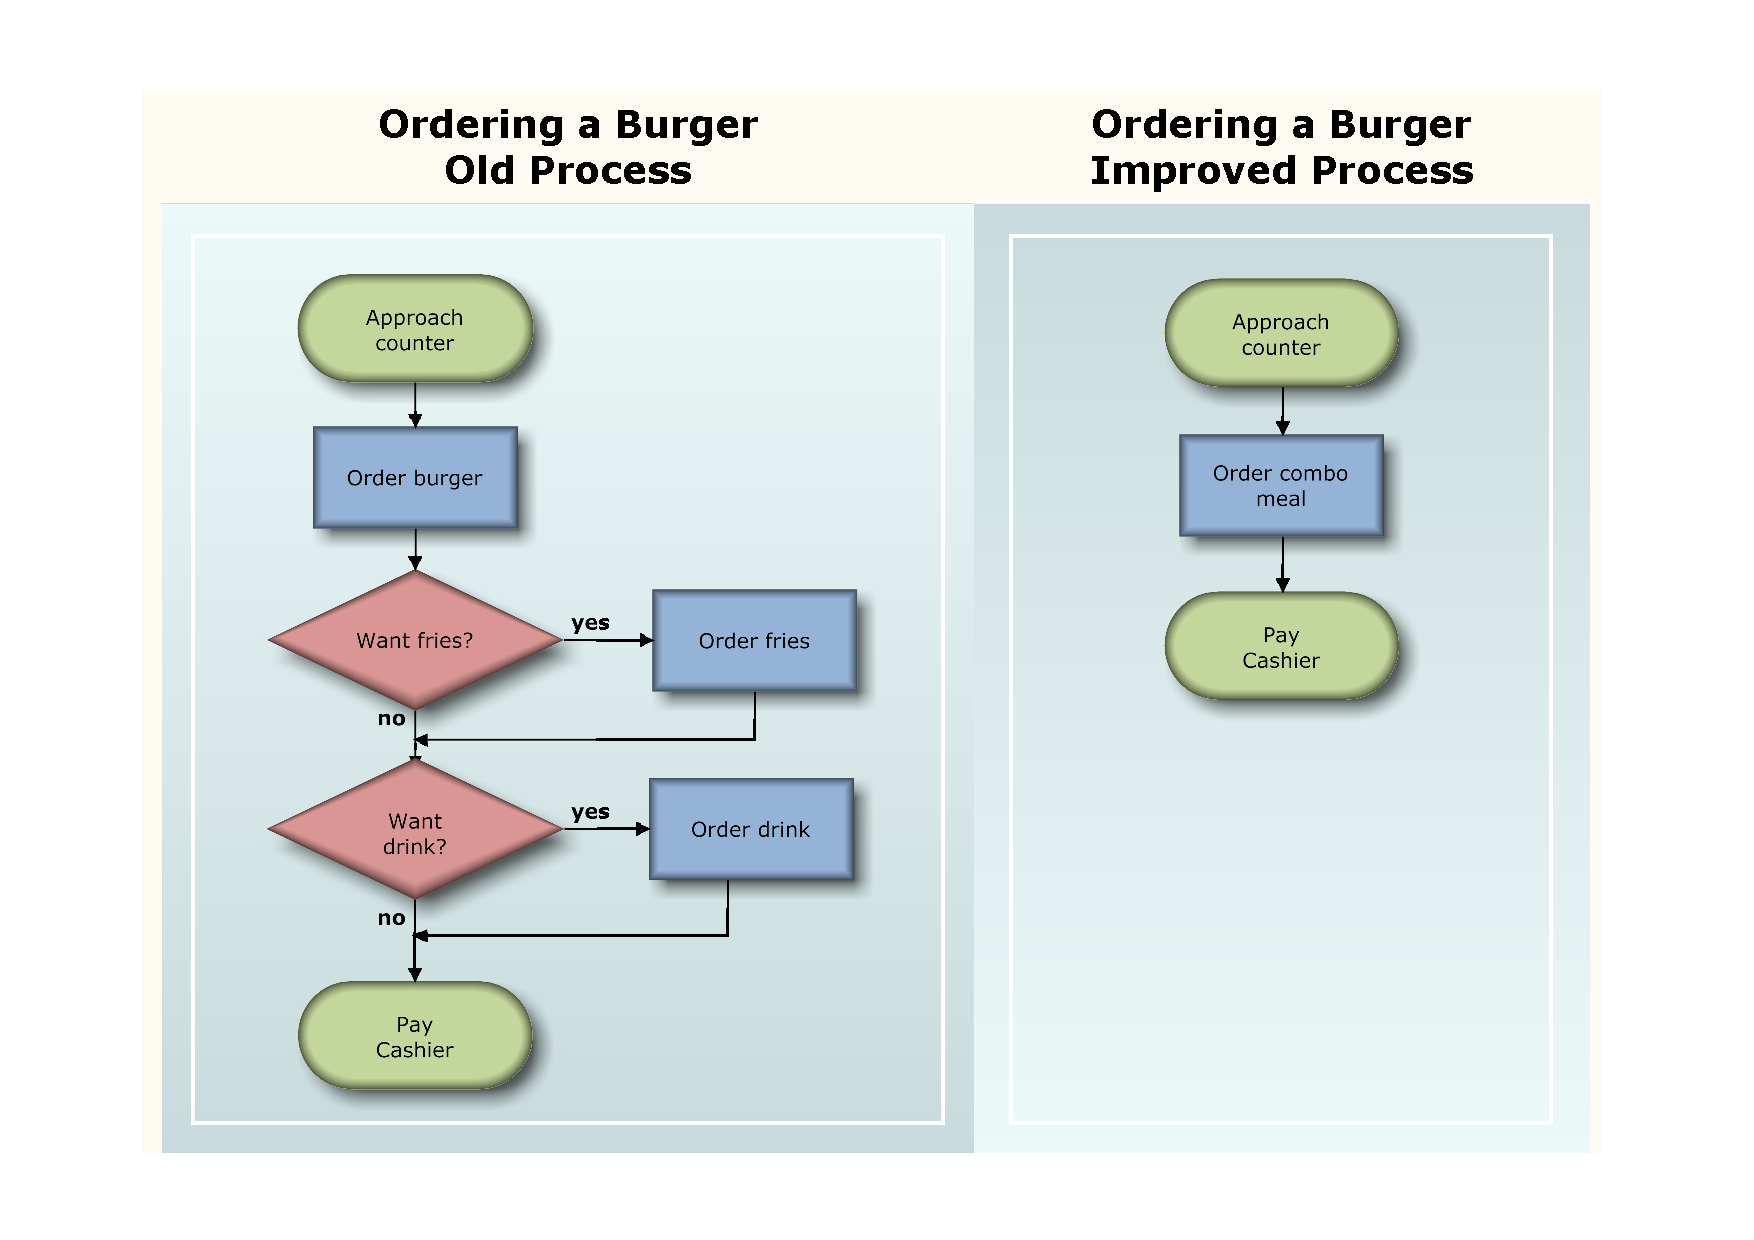
\includegraphics[scale=.6]{BurgerFlowchart}\\ % PDF-File
  \caption{Donec tempor leo a massa~\cite{praxisbuch2017} (Zitat aus Norm, Handbuch u.ö.)}\label{fig:BurgerFlowchart}
\end{figure}

Quisque ligula orci, accumsan vel, molestie ac, lacinia non, lorem . Fusce nonummy. Cras mattis, elit ac tempor congue, ante arcu porta justo, at rhoncus sapien erat vel dui~\cite{latexbib}. Phasellus vestibulum, turpis non tempor vehicula, quam lacus accumsan dolor, id dictum magna magna eu neque. Sed suscipit placerat odio. Sed et sem. Mauris vel tortor a nisl egestas vulputate. Aliquam facilisis luctus nibh. Maecenas vel lectus sed urna viverra pretium. Aenean malesuada nibh sed ipsum. Fusce vel augue. Mauris eget massa. Class aptent taciti sociosqu ad litora torquent per conubia nostra, per inceptos hymenaeos. Etiam nec justo eu purus ultricies mattis. In leo ante, adipiscing sit amet, ultrices at, ultrices et, nulla. Mauris quis odio. Donec sollicitudin rutrum sapien. Aliquam eget ante a dui euismod porttitor. Donec commodo scelerisque purus. Sed magna.\ac{DFN}

\section{Vorgehen und Aufbau}

Der Aufbau der Arbeit ausformuliert.

Nullam consectetuer risus vitae orci. Aliquam fermentum leo sit amet nulla laoreet hendrerit. Maecenas tempus, neque eu posuere vestibulum, pede eros adipiscing augue, pulvinar ullamcorper lectus lectus et tellus. Donec at velit at velit pellentesque sagittis. Vestibulum ultricies ultrices mi. Vestibulum accumsan dictum ligula. Ut lobortis, odio ut semper vehicula, nibh quam semper nisi, sed adipiscing purus lectus et sem. Mauris nisl est, scelerisque ut, ultrices nec, faucibus vitae, nulla. Nulla nisi. Suspendisse potenti. Etiam ultrices commodo odio. Quisque turpis purus, mollis sed, pretium quis, volutpat et, neque. Nam a sapien eget neque consectetuer ornare. Pellentesque felis metus, pellentesque quis, volutpat rhoncus, laoreet id, nunc. Duis egestas, felis et luctus vestibulum, velit nunc luctus felis, non tempor justo ligula et nulla. Vestibulum, Abbildung~\ref{fig:tabelle}, est. Nulla aliquam eleifend justo.


\begin{table}[htb]
  \centering
  \begin{tabular}{|l|c|}
    \hline
    \textbf{tempus} & \textbf{risus} \\ \hline
    ultrices & pellentesque \\
    rhoncus & egestas \\
    \hline
  \end{tabular}
  \caption{Aliquam fermentum}\label{fig:tabelle}
\end{table}

\endinput
